\documentclass[10pt,twocolumn,a4]{article}
\usepackage{styles/usenix-style}
\usepackage{styles/ka-style}
\usepackage{xspace,ifthen,graphicx,listings}
\usepackage{styles/ka-style}

\usepackage[utf8]{inputenc}
\usepackage[inline]{enumitem}
\usepackage{parskip} % disable indentation for new paragraphs, increased margin-bottom instead
\usepackage[english]{babel}
\usepackage{csquotes}
\usepackage[style=alphabetic]{biblatex}
\addbibresource{literature.bib}

\usepackage[
   pdfauthor={Christian Schwarz},
   pdftitle={Seminar Report - Light-Weight Contexts},
   pdfsubject={An OS Abstraction for Safety and Performance}, 
   pdfkeywords={}
]{hyperref}

\setlength{\marginparwidth}{2cm} % to make todonotes fit in twocolumn
\usepackage{todonotes}

\usepackage{blindtext}

\usepackage{listings}
\lstdefinestyle{lwcapi}{language=[ANSI]C,basicstyle=\ttfamily,basewidth=0.5em,fontadjust=true}
\lstset{style=lwcapi}

\usepackage{diagbox}
\usepackage{multirow}

\begin{document}
\title{%
  % document class article doesn't support subtitles, let's hack them
  {\normalfont \normalsize Seminar Report on}\\%
  Light-weight Contexts\\%
  {\normalfont \normalsize An OS Abstraction for Safety and Performance}\\%
  {\normalfont \small %
    James Litton\textsuperscript{1,2}
    Anjo Vahldiek-Oberwagner\textsuperscript{2}
    Eslam Elnikety\textsuperscript{2}
    Deepak Garg\textsuperscript{2}
    Bobby Bhattacharjee\textsuperscript{1}
    Peter Druschel\textsuperscript{2}
  }\\
  {\normalfont \small
    \textsuperscript{1}University of Maryland, College Park 
    \textsuperscript{2}Max Planck Institute for Software Systems
  }%
}
\author{Report by Christian Schwarz}
\date{2019}

\maketitle

\begin{abstract}
  \blindtext\todo{fix blindtext}
\end{abstract}

\section{Introduction}\label{intro}

% TODO NICE SUMMARY OF WHAT LWCs PROVIDE, CAN WE USE THIS ANYWHERE?
%Light-weight contexts can be used to create multiple protection domains within a single process,
%each with a private \textit{address space}, \textit{file descriptor table} and the system \textit{credential} and private per-thread logical control-flow %state (section~\ref{design:createdestroy}).
%Switching between the domains and single-value argument passing is controlled by the kernel (section~\ref{design:switching}).
%Dynamic sharing of resources between lwCs is also kernel-controlled using access capabilities (section~\ref{design:overlays}).
%Access to global namespaces \& system resources (IP sockets, filesystem, IPC) is limited by the lwC's \textit{credential} and can be further controlled %through syscall interposition (section~\ref{design:syscallinterpos}).
%
%Kernel-controlled switching between lwCs results in \textbf{well-defined entry points} under the assumption of an lwC created using \lstinline{COPY} resource %specifier\todo{this is quite coarse, AS and FDT sufficient?}:
%the first \lstinline{lwcSwitch} diverts physical control flow to the \lstinline{lwcCreate} call site in the new lwC, and all subsequent \lstinline{lwcSwitch}%es resume execution at an lwcSwitch all site.
%Under the assumption of no dynamic sharing, the address space of the target lwC is inaccessible to any caller.
%Thus, integrity and confidentiality guarantees for code and data within an lwC are those of the application code creating the lwC and those of the code %executing in the target lwC after \lstinline{lwcSwitch}.
%The result is a narrow, auditable interface.
%

Modern application architecture emphasizes modularization and information hiding to achieve testability, maintainability, exchangability, and reusability.
The extreme of reusability are large libraries that are used by multiple independent applications.
Type systems, packaging hierarchies, and visibility features in many programming languages can help to enforce said principles in large applications.

However, there is a chasm between the way we architect software and the way it is executed it at runtime:
whereas the programming language enforces strict separation between modules on the type level at compile time,
the program binary or interpreted script executes in a single protection domain --- the process ---
with shared address space, file descriptor table and system-level privilege for all modules.
Consequently, an exploitable vulnerability in a single logical module can be used to compromise the entire application, extract user data from application memory or serve as a basis for further privilege escalation.

Language technology provides holistic solutions to this problem through memory-safe languages, runtime ACL systems, etc.
However, performance concerns, lack of interoperability between different source languages within a process, and legacy code bases shift the search for better runtime safety guarantees toward the next lower layer of the software stack:
Can the operating system provide an efficient abstraction to maintain some of the aforementioned compile-time isolation at runtime?

Light-weight contexts (lwCs) are such an OS-based solution that allows for multiple protection domains (\textit{contexts}) within the same process:
An lwC is comprised of an address space, file descriptor table and system credential (privilege level).
In contrast to the implicit execution environment provided by a process, lwCs are a first-class OS abstraction and explicitly tangible from user space as file descriptors.

In the proposed design, threads no longer execute a single logical control flow, but have one \textit{per lwC}.
A new system call allows for rapid voluntary switching to a different lwC: apart from resuming the thread's target lwC logical control flow, the system call also installs the target lwC's address space, file descriptor table and system credential for the current thread.
Argument passing on switch then enables the decomposition of an application's functionality into multiple lwCs that can provide independent security guarantees.

Further, the lwC design describes the mechanisms for creating lwCs within a process which allows for selective sharing of memory, file descriptors and privilege level.
Dynamic sharing of these resources is also supported through a capability system built on top of lwC file descriptors.
Privelege escalation through out-of-process channels can be prevented using syscall interposition, which enables efficient program-defined policy enforcement for syscalls made by an lwC.

The authors provide an evaluation of their implementation in FreeBSD 11.0, focussing on the enhancement of inter-request isolation and TLS private key protection in web servers.
Whereas the presented results are impressive at first glance, we find that the evaluation lacks key metrics for the presented use cases and does not sufficiently investigate obvious performance-constraints of the design.

% Generic questions / problems / tradeoffs:
% \begin{itemize}
  % \item threat model
  % \item definition of what makes a protection domain
  % \item how to integrate the decomposition into different protection domains into the PL / runtime?
  % \item applicability to existing PLs \& code bases
  % \item how to maintain application performance
% \end{itemize}

\subsection{Structure of this Report}
This report provides a summary of the original light-weight context paper enriched with several insights drawn from the author's open source implementation.
Section~\ref{design} provides an overview of the design and system API exposed by lwCs,
followed by a brief security analsys in section~\ref{security}, which also includes an example use case for\todo{of?} lwCs in application security hardening.
We briefly discuss the author's implementation of lwCs in FreeBSD 11.0 in section~\ref{impl} and then proceed with a discusion of the evaluation results of the original paper (section~\ref{eval}).
Subsequently, we survey other approaches to application compartmentalization in section~\ref{rel}.
Finally, we provide an elaborate critique of the design \& evaluation in section~\ref{eval:crit}.

\section{Design}\label{design}
We find it most helpful to develop the general idea of \textit{light-weight Contexts} (lwCs) by starting from the canonical abstraction of processes \& threads, as visualized in figure~\ref{design:fig:canonicalprocthreads}.
\begin{figure}
  \label{design:fig:canonicalprocthreads}
  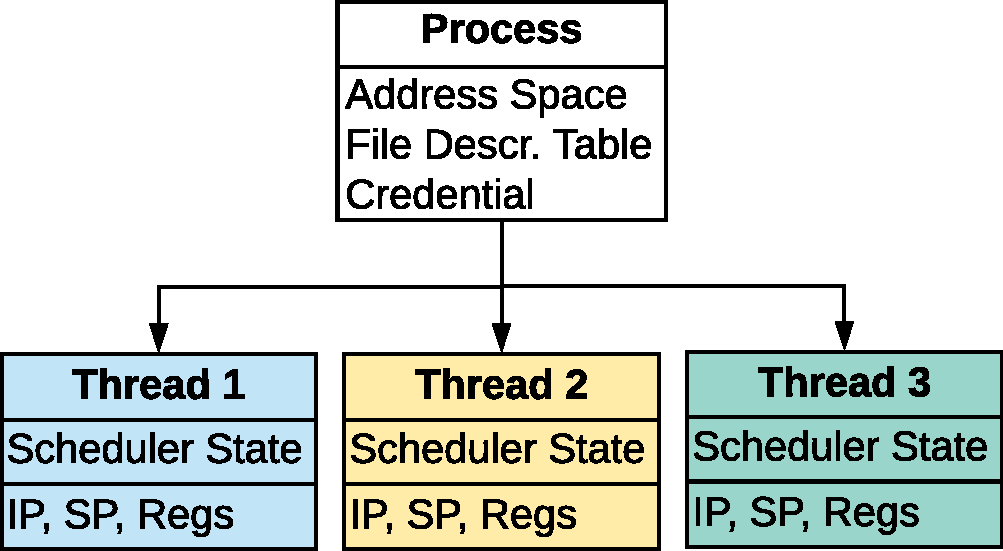
\includegraphics[width=\linewidth]{fig/canonical-proc-thread-relationship}
  \caption{
    Canonical state associated with processes and threads and the relationship between them.
    The process implicitly defines the execution environment for threads.
    Threads are scheduling entities that represent a single control flow bound to the process-defined environment.
  }
\end{figure}
Conventionally, processes define an execution environment which is shared by one or more threads.
The execution environment consists of an address space, a file descriptor table and a representation of the process's system-wide privileges (\textit{credential}).
A thread has \textbf{two closely related, but separate roles}:
\textbf{first}, it represents a \textbf{single unit of logical control flow} within the process-defined environment.
Control flow has associated state, e.g., instruction pointer, stack pointer, general purpose register contents, FPU state, etc.
That state resides in a CPU's registers while the thread is executing on a CPU, or in the thread control block (TCB) kernel data structure.
The \textbf{second} role of a thread is that of a \textbf{scheduling entity}:
The scheduler time-multiplexes threads onto CPU cores and implements the concept of blocking \& waiting between threads.
The scheduler state required for this task is stored in the thread control block (TCB).

The authors introduce light-weight contexts as a new OS abstraction and restructure the roles of canonical processes \& threads, as visualized in figure~\ref{design:fig:lwcprocthreadrelationship}:

\begin{figure}[h]
  \label{design:fig:lwcprocthreadrelationship}
  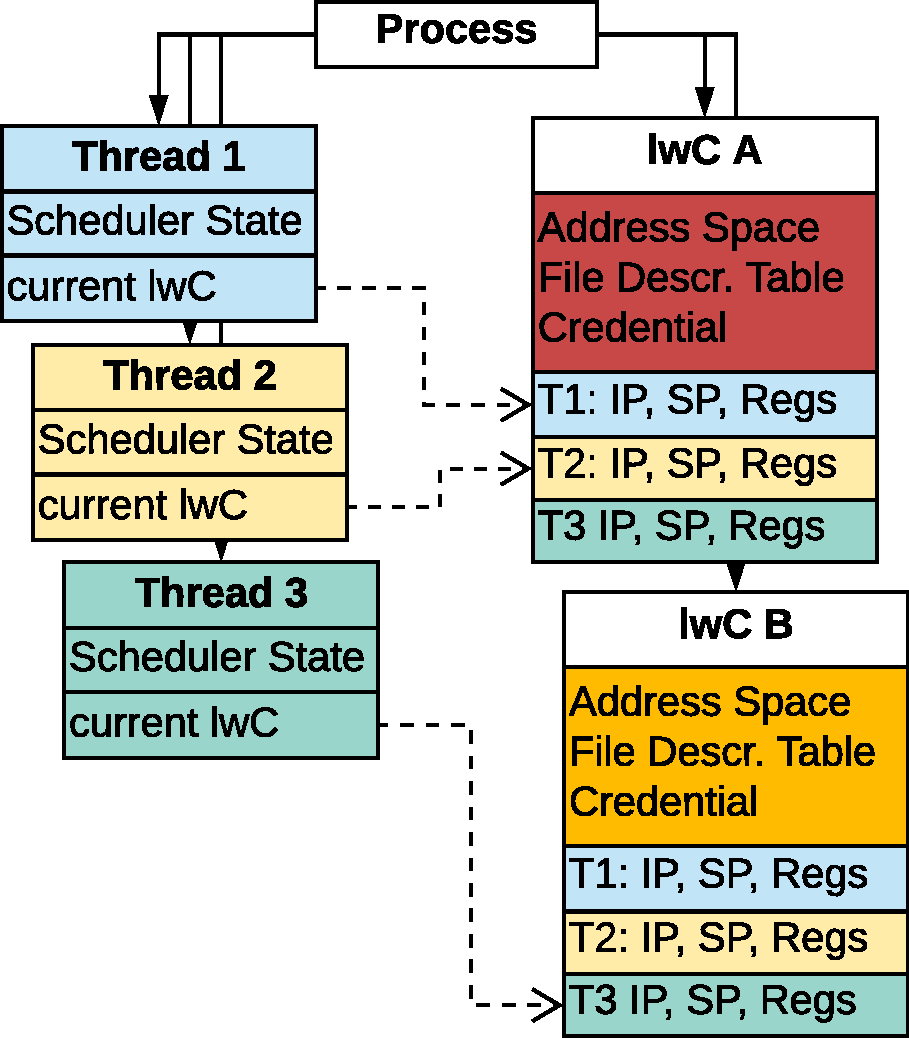
\includegraphics[width=\linewidth]{fig/lwc-proc-thread-relationship}
  \caption{
    State associated with lwCs, processes and threads and relationships between them.
    Processes act as containers for threads and lwCs.
    Threads are reduced to their role as scheduling entities.
    Each lwC represents an execution environment and holds control flow state for each thread.
  }
\end{figure}

\begin{itemize}
\item An lwC represents a single protection domain (address space, file descriptor table and system credential) and all logical control flows within that protection domain.
\item Threads always execute within one lwC at any given time and always execute the same logical control flow while within that lwC.
\item Multiple threads can execute simultaneously within an lwCs, sharing a protection domain but executing different logical flows.
\item lwCs are represented as file descriptors, and thus explicitly tangible from user space.
\item Threads can switch protection domains and logical control flow by switching between lwCs.
\end{itemize}

In the following subsections, we provide an outline of the system API for managing and using lwCs in an application.
Subsequently, we summarize the security guarantees provided by lwCs and provide usage examples for this new OS abstraction. 

\subsection{lwC Switching}\label{design:switching}
We start our survey of the lwC API surface with the most central functionality: switching between lwCs.
We accept the existence of multiple lwCs for now and come back to lwC creation in the next subsection.

Threads can switch between lwCs by invoking the \lstinline{lwcSwitch} system call:

\begin{lstlisting}[float=h]
  caller, carg := lwcSwitch(target, arg) 
\end{lstlisting}

The first argument \lstinline{target} specifies the file descriptor of the lwC into which the calling thread wants to switch.
When invoking the system call, the kernel
\begin{enumerate}[label=(\alph*)]
\item saves the current control flow state into the current thread's lwC,
\item atomically switches to the new protection domain by installing the target lwC address space, file descriptor table and credential for the current thread,
\item and restores the control flow state saved for the current in thread in the target lwC.
\end{enumerate}
Pseudo code for this procedure is provided in listing~\ref{design:fig:switchpseudocode}.

\begin{lstlisting}[mathescape,label=design:fig:switchpseudocode,caption=Pseudo code for lwcSwitch.,frame=trbl]
  syscall
  
  SP, IP, $\dots$ $\rightarrow$ curLWC->tcb[tid]
  
  curThd->vmspace = targetLWC->vmspace
  curThd->fdt = targetLWC->fdt
  curThd->cred = targetLWC->cred
  curLWC = targetLWC
  
  SP, IP, $\dots$ $\leftarrow$ targetLWC->tcb[tid]
  (arg kept in register)
  
  sysret  
\end{lstlisting}
  
It is crucial to understand that \textbf{execution after a switch always resumes at an lwC call site}, except for the very first switch into a newly created lwC (see section~\ref{design:createdestroy}).
Note that this behavior is analogous to a voluntary context switch, e.g., with \lstinline{pthread_yield}.
However, in contrast to the canonical model of processes \& threads, \textbf{\lstinline{lwcSwitch} does not switch to another scheduling entity}:
from the thread scheduler's perspective, it is still the same thread that is executing on the CPU.
In fact, \textbf{the thread scheduler is not affected at all by lwC switching}:
it still handles context switches post-interrupt, post-exception or when a thread blocks, by simply saving that thread's control flow state to the slot in the current lwC before switching to another thread (i.e.~scheduling entity).

The second argument to \lstinline{lwcSwitch} is an opaque value called \lstinline{arg} that is passed through to the code that starts executing in the target lwC after the switch is completed.
\lstinline{arg} is made available in the target lwC as the return value \lstinline{carg} (we remember that execution always resumes at an lwC call site).
The second return value \lstinline{caller} is the file descriptor of the lwC from where the switch was initiated.

Note that these three properties of lwcSwitch --- kernel-moderated control flow switching, address space switching, and argument passing --- enable the construction of lwCs that fulfill a server-like role within an application, providing independent security properties:
as will be discussed in section~\ref{design:usage}, one lwC can provide some high-assurance service to other lwCs because it has a private address space and can enforce specific entry-points (\lstinline{lwcSwitch} call sites) where argument validation can be performed.

\subsection{lwC Creation \& Destruction}\label{design:createdestroy}
A process in an lwC system starts with a single thread that runs within a root lwC created by the OS.
This design enables backwards binary-compatiblity with the exception that the root lwC file descriptor is a well-known number analogous to those for stdio.

New lwCs can then be created by threads using the \lstinline{lwcCreate} system call:

\begin{figure}[h]
  \centering
\begin{lstlisting}[mathescape]
  new, caller, carg := lwcCreate(rspecs)
\end{lstlisting}
\begin{tabular}{|r||c|c|c|}
  \hline
                &   new        & caller       & carg \\
  \hline\hline
  creator       & new lwC fd   & $\bot$      & $\bot$\\
  \hline
  new lwC       &    creator lwC fd   & \multicolumn{2}{c|}{like lwcSwitch}\\
  \hline
\end{tabular}
\caption{
  \texttt{lwcCreate} return values are different in creator and new lwC to ensure well-defined behavior when the creator switches to the new lwC for the first time.
}
\end{figure}

By default, a new lwC is a snapshot of the calling thread's current lwC, as depicted in figure~\ref{design:fig:lwccreationsequencediagram}:
The kernel first creates copies of the resources \textit{address space}, \textit{file descriptor table} and \textit{credentials} and stores them in the new lwC.
It then temporarily preempts all threads that execute in the current lwC and stores their control flow state in the new lwC.
The execution state of other threads that can switch to the creating lwCs is simply copied to the new lwC.
Finally, the file descriptor referring to the new lwC is returned to user space in the return value \lstinline{new}.

\begin{figure}
  \centering
  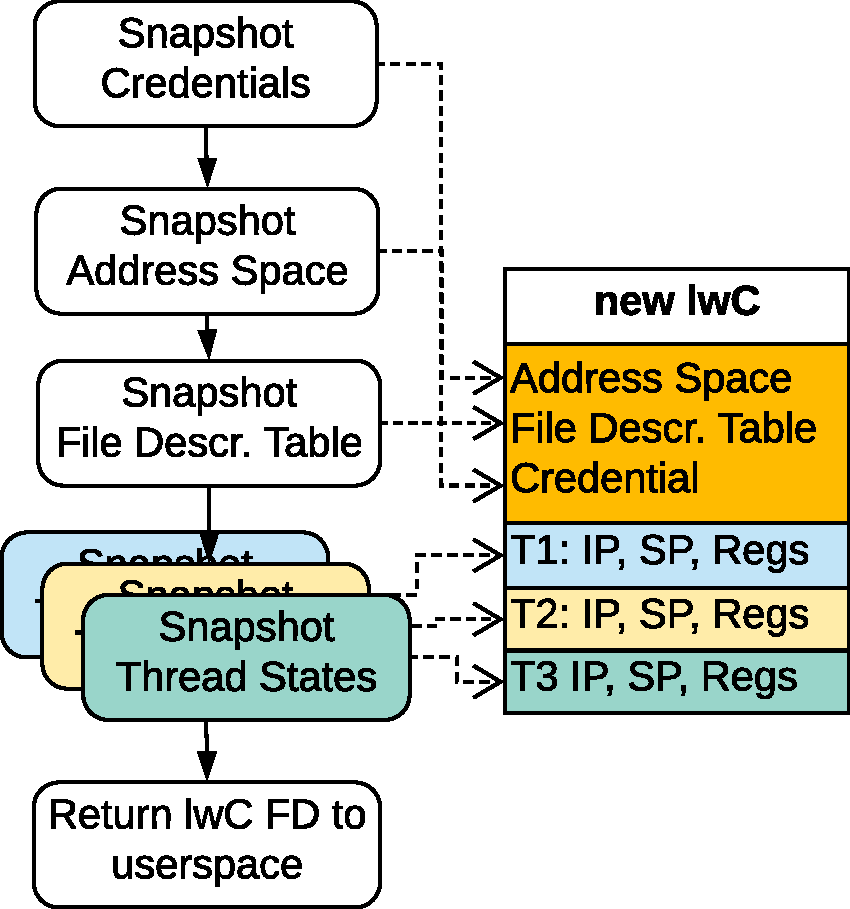
\includegraphics[height=4cm]{fig/lwc-creation-sequence-diagram}
  \caption{
    Steps involved in lwC creation.
    By default, a new lwC is a copy (snapshot) of the current lwC's resources.
    All threads that exist at the time of lwC creation can enter the new lwC.
  }
\label{design:fig:lwccreationsequencediagram}
\end{figure}

Note that in contrast to the original paper, we avoid the term \textit{fork} when describing the lwC creation procedure:
forking has the same resource snapshotting semantics as \textit{lwcCreate}, but also implies the creation of a new process and scheduling entity.
In contrast, \textit{lwcCreate} only creates a copy of the protection domain and a handle for existing threads to switch to it later --- no independent scheduling entity is created.

However, one problem of forking translates to lwC creation:
\textbf{what happens when we first switch into a newly created lwC? How does snapshotting interact with multi-threading?}
After all, we preempt and snapshot all threads' control flow states on lwC creation, and the \lstinline{lwcSwitch} implementation restores that state on first switch, expecting that it was an \lstinline{lwcSwitch} call site.
We need to consider two cases:
the \lstinline{lwcCreate}ing thread will appear return "a second time" from that syscall and populate \lstinline{lwcCreate}'s \lstinline{caller} and \lstinline{carg} return values with those of \lstinline{lwcSwitch}.
Additionally, the \lstinline{new} contains the lwC descriptor of the creator lwC.
The behavior in the creating thread is thus well-defined.
Other threads could be at random points in their logical control flow when being snapshotted, resulting in undefined behavior after the switch.\todo{obvious?}
Multithreaded forking is a well-known problem, \todo{citation} and the authors recommend applications to use barrier-synchronization with the creator.\todo{cite}
However, it is unclear to us how the \lstinline{caller} and \lstinline{carg} return values are accessible without inline-assembly or language support for non-creator threads.\todo{check}

Finally, it should be noted that a new lwC only stores control flow states for the threads that existed at the time of its creation:
threads created after the lwC cannot switch into the lwC.

\subsubsection{lwC Resource Specifiers}\label{design:rspecs}
The previous section presented the default behavior of \lstinline{lwcCreate} for an empty \lstinline{rspecs} argument, which amounts to the new lwC being a snapshot copy of the current lwC's \textbf{resources} \textit{address space}, \textit{file descriptor table} and \textit{credential}.
By using \textit{resource specifiers}, the application can control resource sharing at a more fine-grained level:
resources of the current lwC can be either \textit{copied to}, \textit{unmapped from} or \textit{shared} with the new lwC.
For address space and file descriptors, different sharing behavior can be specified on a per-page or per-descriptor basis.
Figure~\ref{design:fig:rspectable} summarizes the different combinations of resources and sharing behavior.

\begin{figure}[h]
  \centering
\begin{lstlisting}
rspecs := [{Resource , [Start, End), How}]
\end{lstlisting}

\begin{tabular}{|r||m{1.5cm}|m{1.5cm}|m{1.5cm}|}
  \hline
  \diagbox[width=5em]{How}{What}    &     Address Space         &         File Descriptor Table         &           Credential           \\
  \hline
  COPY                              &   copy on write sharing           &      \texttt{dup} open FDs once    &  copy credential kobject  \\
  \hline              
  UNMAP                             &   do not map              &       do not \texttt{dup} FDs         &    $\bot$       \\
  \hline              
  SHARE                             &   shared memory            &   share kobject   &             share kobject   \\
  \hline
\end{tabular}
\caption{
  Resource specifiers change the default snapshot semantics of \texttt{lwcCreate}:
  each resource can be copied, shared or unmapped from the new lwC.
  Address space and file descriptor sharing can be configured per page / per descriptor.
  \textit{copy} sharing is roughly equivalent to what happens on \texttt{fork}, \textit{share} to what happens on thread creation.
  }
\label{design:fig:rspectable}
\end{figure}
\todo{language, prettier table}

\subsection{Dynamic Resource Sharing with lwC Overlays \& Access Capabilities}\label{design:overlays}
Apart from sharing at lwC creation time, it is also possible to dynamically copy or share memory and file descriptors between lwCs or to temporarily escalate system privileges to the credential of another lwC through the \lstinline{lwcOverlay(src, rspecs)} system call.
The \lstinline{src} argument is the file descriptor of the lwC from which the subset of resources specified in \lstinline{rspecs} should be mapped (\textit{overlaid}) into the current lwC.
The target address (for memory overlays) or file descriptor number is guaranteed to be the same as in \lstinline{src}.
To unmap an existing overlay, \lstinline{src} must be set to the current lwC and \lstinline{rspecs} must be filled with \lstinline{UNMAP} resource specifiers. 
Overlays do not support stacking: after unmapping an overlay that overlaid an existing memory mapping, that original memory mapping is not automatically remapped.\todo{proof by code}  %vmspace_lwc_merge

Overlaying resources from an lwC descriptor \lstinline{src} further requires that this descriptor is equipped with \textbf{access capabilities} for each requested resource.
The rules of this capability system are as follows:
\begin{itemize}
  \item After lwC creation, the creator receives the \lstinline{new} lwC descriptor with a universal access capability to the child lwC.
  \item After lwC creation, the child receives the lwC descriptor of its creator in \lstinline{new}, equipped with access capabilities to ranges flagged with \lstinline{LWC_MAY_ACCESS} on lwcCreate.
  \item Access capabilities cannot be extended.
  \item Access capabilities can be reduced with the \lstinline{lwcRestrict(target, rspecs)} system call by any lwC that holds the lwC descriptor \lstinline{target}:
        after a successful \lstinline{lwcRestrict}, the resource ranges specified in \lstinline{rspecs} can no longer be overlaid using \lstinline{lwcOverlay(target, ...)}.
  \item Access capabilities are invariant across overlays: to the file descriptor entry in the kernel, and is therefore invariant across overlays.
\end{itemize}

In order to grasp the access capability system, we find it helpful to peek at the authors' implementation.
The access capabilities associated with an lwC descriptor are represented as an \lstinline{rspecs} in lwC file descriptor table entry (\lstinline{struct filedescent}).
The overlay permission check enforces that the requested overlay rspec is a subset of the rspec in that file descriptor table entry.

Note that revocation of existing overlays is not possible, i.e., \lstinline{lwcRestrict} only affects future overlays.\todo{proof, not mentioned in paper / impl. see microkernel discussions}

\subsection{Syscall Interposition in Capability Mode}\label{design:syscallinterpos}
% kernel: lwctrapto in sys/kern/subr_syscall.c basically just calls lwcswitch 
When compartmentalizing an application into different lwCs, it can be desirable to limit the system calls an lwC may perform, e.g., to limit filesystem access to a subdirectory or prohibit network communication.
The lwC design builds onto existing syscall filtering and mechanisms, e.g. Capsicum capability mode on FreeBSD or seccomp on Linux\todo{cite}:
when an lwC is created with the \lstinline{LWC_TRAP_SYSCALL} flag, system calls made by the new lwC or any of its children that would normally trap due to the syscall filtering mechanism are redirected to the creator as an \lstinline{lwcSwitch} with \lstinline{caller} set to the trapping lwC.
After the trap-handling lwC has evaluated its policy, the \lstinline{lwcSyscall} system call provides the mechanism for the trap-handling lwC to execute any system call (the original one, another one) \textbf{in the context of the trapping lwC}:

\begin{lstlisting}[float=h]
  lwcSyscall(trappingLwc, mask,
             syscall, syscall-args)
\end{lstlisting}

An alternative design could require the trap-handling lwC to invoke the allowed syscalls itself and return the result as the opaque argument in an \lstinline{lwcSwitch} to the trapping lwC.
However, if the syscall arguments contain pointers to user memory or file descriptors, the trap-handling lwC would need to overlay those from the trapping lwC.
\lstinline{lwcSyscall} avoids the associated overhead:
the \lstinline{mask} argument allows the trap-handling lwC to choose per resource type\footnote{granularity: all memory, all file descriptors, the credential} whether its own mapping or that of the trapping lwC should be used while the syscall is executed.


\subsection{Signal Delivery}
UNIX signal delivery with lwCs faces the same design questions as with threads, i.e., to which lwCs a given signal should be delivered.
The authors' solution is to classify signals as either \textit{attributable} or \textit{non-attributable}:
attributable signals such as for segmentation faults are always delivered to the thread in the lwC that caused the signal to occur.
Non-attributable signals are delivered to \textit{all} lwCs created with a corresponding flag.
Consequently, each thread must have a separate signal mask per lwC.\todo{verify in src}

\subsection{Forking \& Exit}
A forked process inherits the parent's lwCs.
However, only the forking thread exists in the child process, presumably due to POSIX compliance\cite{forkmultithread}. %read do_fork, which calls copy_snaps
Shared memory, either through resource-specifiers on \lstinline{lwcCreate} or \lstinline{lwcOverlay} or through \lstinline{mmap(..., MAP_SHARED)} stays shared accross forks.
The authors do not specify the behavior for file descriptor tables and credential; we assume unmodified fork semantics per lwC.

\subsection{Summary}

\todo{TODO}
% TODO TODO TODO TODO TODO TODO TODO TODO TODO TODO TODO TODO TODO TODO TODO TODO TODO TODO TODO TODO TODO TODO TODO TODO 
\begin{figure}[h] % TODO make this a broad figure?
\centering
\begin{tabular}{|r|m{1.5cm}|}
  \hline
  lwcCreate & \\
  \hline
  lwcClose & \\
  \hline
  lwcGetLwc & \\
  \hline
  lwcSwitch &  \\
  \hline
  lwcOverlay & \\
  \hline
  lwcRestrict & \\
  \hline
  lwcSyscall & \\
  \hline
\end{tabular}
  \caption{lwc API summary table}
\end{figure}


\section{Security Analysis}\label{security}

In this section, we define a threat model for lwCs and assess how the design meets the canonical information security properties of \textit{confidentiality}, \textit{integrity} and \textit{availability}\cite{ciagoals}.

\textbf{Threat Model}\hspace{1em}
The run-time trusted computing base of a process that uses light-weight contexts is the
hardware,
firmware,
monolithic OS kernel,
any user space processes able to influence the execution \& environment of the lwC-process,
and any user space code that runs before \lstinline{main} starts executing.
Once \lstinline{main} starts executing, we assume an attacker who is able to hijack control flow and execute arbitrary code in user-mode in the currently established execution context, i.e., the current lwC.
Specifically, an attacker may access any mapped memory through unprivilieged instructions and invoke any system call, including lwC management calls, and attempt privilege escalation directly or indirectly by invoking said system calls.

\textbf{Resource Mappings}\hspace{1em}
An lwC consists of resource mappings for the three resource kinds address space, file descriptor table and credential.
The kernel implementation of \texttt{lwcSwitch} must guarantee that all kernel subsystems as well as the memory management unit will always perform their respective access permission checks against the resource mappings of the lwC that was last switched to, i.e., the current thread's current lwC.
Under that assumption, the lwC security guarantees rely solely on the soundness of the rules by which resource mappings can be manipulated from user space through \lstinline{lwcCreate}, \lstinline{lwcRestrict} and \lstinline{lwcOverlay}, as well as their correct implementation.
Note that neither the original paper's authors nor us provide a proof of soundness of the resource mapping manipulation.

The \lstinline{lwcSyscall} API must be considered separately:
its \lstinline{mask} argument allows the trap-handling lwC to specify a \textit{subset} of resource mappings to be established for the duration of the syscall.
This differs from \lstinline{lwcSwitch}, which only allows switching \textit{all three resource mappings} atomically before executing code in the context of the target lwC.
We therefore demand that it must not be possible to extend the set of \textit{passing} permission checks in kernel or memory management unit by invoking \lstinline{lwcSyscall} with a \lstinline{mask} that combines resource mappings from trapping and trap-handling lwC, compared to invoking the syscall directly from either the trapping or the trap-handling lwC.


\textbf{Achieving Protection Goals}\hspace{1em}
Applications must create lwCs with correct resource mappings and access capabilities in order to achieve their desired protection goals.
For example, full confidentiality and integrity of a region of memory in the root lwC can be achieved by asserting that any child lwC is created with a resource specifier that marks that region as \lstinline{UNMAP}ed.
\textit{Loop holes}\todo{language} such as attaching a debugger to the parent lwC from the child lwC must also be addressed, e.g., through system call interposition or by dropping privileges in the child lwC.

It is evident that given a tree of lwCs created with \lstinline{lwcCreate}, access rights to resources of parent lwCs from child lwCs do monotonically decrease under the absence of dynamic resource sharing.
Conversely, the use of dynamic sharing prohibits such general statements about access rights between lwCs because the dynamic flow of lwC file descriptors at runtime cannot always be statically predicted.

Availability cannot be guaranteed by lwCs:
an attacker in control of an lwC may invoke the \lstinline{exit} system call to terminate the process unless syscall interposition is used to prevent that syscall.
An attacker may also modify the code in a compromised lwC to block indefinitely or never invoke \lstinline{lwcSwitch}, effectively trapping all threads that switch to the compromised lwC.
The authors dismiss both problems by describing denial-of-service (DoS) within a process as "self-defeating".\todo{quote}
We remark that the original paper does not address per-lwC resource usage (limits), which could serve as another DoS vector. 


\subsection{Example Use Case: Application Compartmentalization}\label{design:usage}

Application developers can leverage lwCs to achieve application protection goals.
We restrict ourselves to a discussion of a fictional application called \newcommand\appname{\textit{convert.io}\xspace} \appname which will use lwC-based \textit{application compartmentalization} to increase confidentiality of user data and its TLS private key. 
\appname is a network service which
\begin{enumerate}
  \item accepts JPEG images over TLS from arbitrary internet clients,
  \item uses an image processing library to convert the image into the client-requested output format and
  \item sends a response with the converted image back to the client.
\end{enumerate}

We consider an attacker who exploits a vulnerability in the image processing library's image codec parser to achieve remote code execution:
in an uncompartmentalized design, a successful attacker can read the entire process's memory to extract the private key of the TLS key pair or access other users' images from other requests.
Both \textit{private key confidentiality} as well as \textit{client session isolation} are compromised.

In contast, an lwC-enabled design loads the TLS private key into the root lwC and waits for connections.
For each new connection, it creates a worker lwC with private copy of the root lwC's address space and file descriptor table and switches into it.
After performing the TLS hand-shake, it erases the private key from the worker address space and, only then, starts executing the riskier image processing code.
A successful attacker now does not have access to the private key and is limited to the socket representing their own connection, as well as their own request data.
A visualization of the two approaches is given in figure~\ref{design:usage:apparchpost}.

\begin{figure}
  \label{design:usage:apparchpre}
  \label{design:usage:apparchpost}
  \centering
  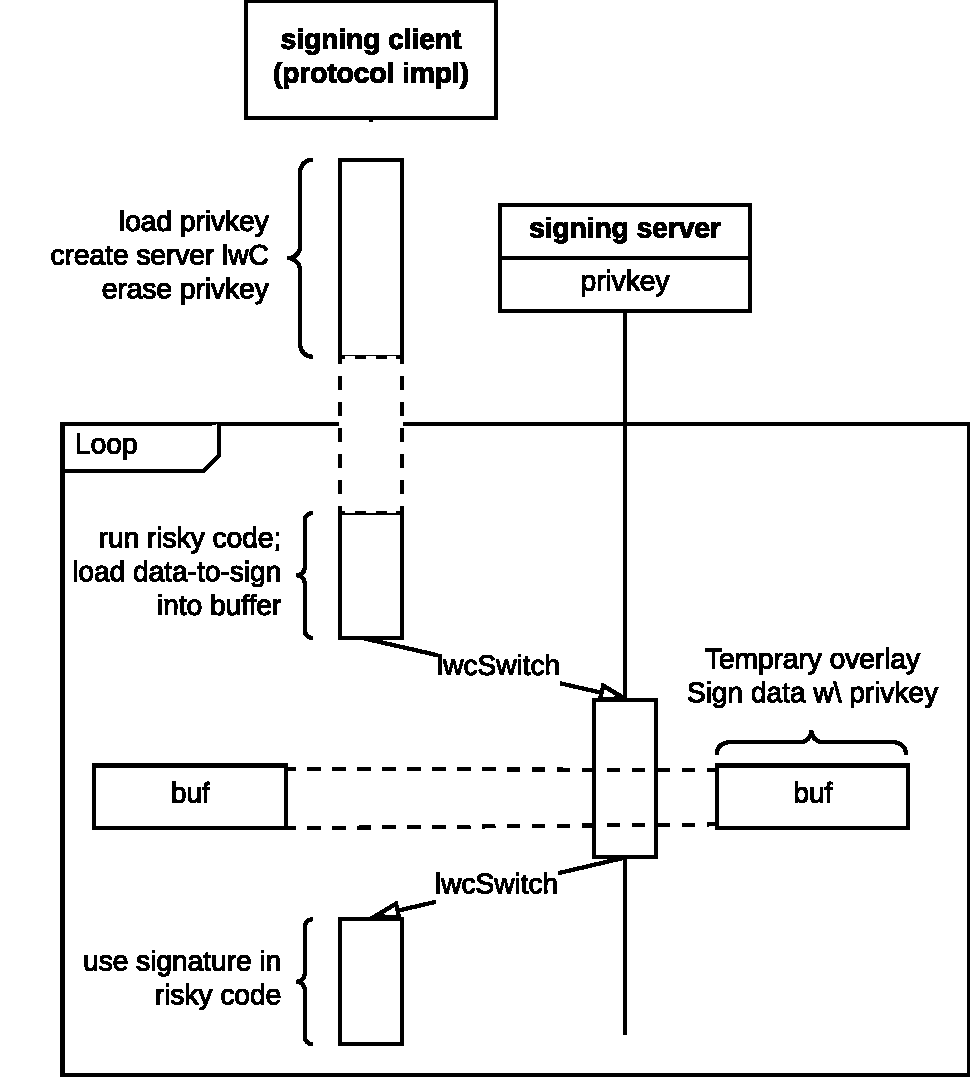
\includegraphics[height=4cm]{fig/encryption-compartment}
  \caption{
    TODO FULL WIDTH a)  b) comparison as described in Example Use Case section
  }
\end{figure}

Note that we have constructed a simplified example where requests can be handled in full isolation.
In practice, some sharing will be required, e.g., for global statistics, a database connection pool, logging services, etc.
In an lwC-compartmentalized design, these components would exectute in separate lwCs and be made accessible to the worker lwCs via shared memory, \lstinline{lwcSwitch}, \lstinline{lwcOverlay} or traditional IPC mechanisms.

Note further that we have not discussed the concurrency model of \appname: both threaded and event-driven models are possible, as will be shown in the evaluation (section~\ref{eval}).


\section{Implementation}\label{impl}

The authors implement light-weight contexts in the FreeBSD 11.0 operating system and make the source code publicly available.~\cite{lwckernelrepo,lwclibsrepo} % see literature.bib for git diff
The major changes to the kernel consist of:
\begin{itemize}
  \item An implementation of syscall handlers and resource specifier logic (+2388 lines in \texttt{sys/sys/kern\_snap.c}).
  \item Support for resource specifiers and overlays in
    file descriptor management (\lstinline{struct filedesc}, +251 lines in \texttt{sys/kern/kern\_descrip.c})
    and memory management subsystem  (+693 lines in \texttt{sys/vm/vm\_map.c}, +178 lines in \texttt{sys/amd64/amd64/pmap.c}).
  \item Platform-dependent code for \lstinline{lwcSwitch} (+250 lines in \texttt{sys/amd64/amd64/cpu\_switch.S}, +171 lines in \texttt{sys/amd64/amd64/vm\_machdep.c}).
\end{itemize}

User-space support for lwCs is provided through a C~library containing syscall wrappers and a synchronized hash-table that enables key-value sharing across lwCs.
The authors also provide a PHP extension that makes the lwC API accessible from scripts, which is requried for the evaluation.~\cite{lwclibsrepo}

\section{Evaluation}\label{eval}
The authors evaluate their implementation using micro-benchmarks to determine the primitive operations' latency
and integrate light-weight contexts into production applications, demonstrating its applicability and real-world performance impact.

\subsection{Micro-Benchmarks}
The micro-benchmarks first measure \lstinline{lwcSwitch} latency with regular context switching as the baseline, demonstrating a 2x speedup with negligible standard deviation.
While not explicitly stated, we assume that the switch is between lwCs with \textit{different} address spaces.
The mechanism used to measure regular context switch latency is a standard POSIX semaphore.

The latency of lwC creation and destruction is only explored cummutatively: creating and immediately destroying a single lwC takes $87.7\mu s \approx 233282$ cycles on the evaluation machine. %(87.7*10^-6) * 2.66*10^9 = 233282
However, the authors do not provide a meaningful baseline, e.g., the latency of a forking and immediately exiting in the child.
An extended version of this micro-benchmark is also used to argue that the direct run-time overhead \textit{within} an lwC is limited to CoW faults.
However, the indirect cost of multiple address spaces (e.g. increased TLB pressure) is neither considered nor evaluated.

The syscall interposition feature is evaluated by example:
the authors implement a reference monitor that intercepts the \lstinline{open}, \lstinline{read} and \lstinline{write} system calls, execute a dummy application that performs a fixed number of those system calls, and measure total execution time.
For comparison, they also measure a variant with inlined policy checks, as well as a variant that uses FreeBSD's Capsicum and multiple processes.
Thus, the result is the \textit{total execution time} per variant and system call, which is only useful to compare \textit{throughput, not latency}.
Expectably, inlined policy checks exhibit the lowest overhead in all cases.
Capsicum and syscall interposition are penalized\todo{language} by the required context in the case of short syscalls like \lstinline{open}, small \lstinline{read} and \lstinline{write}.
For longer syscalls (large \lstinline{read}, \lstinline{write}), syscall interposition benefits from the \lstinline{mask} argument because --- unlike Capsicum --- copying the buffer to the reference monitor is not necessary.
\todo{figure helpful?}

\subsection{Application I: FastCGI Acceleration in PHP-FPM}
The first application benchmark uses light-weight contexts within the PHP-FPM FastCGI server to reduce interpreter and application initialization time, using a technique called \textit{snapshot-and-rollback}:
on first startup, before handling any request-specific data, the PHP script creates a snapshot of its initialized state using \lstinline{lwcCreate}.
This snapshot is then used as the basis for handling subsequent requests in a separate isolated lwCs which start execution at the pre-initialized state of the original snapshot.
Pseudocode for this operation is provided in figure~\ref{eval:phpfpm:pseudocode}.

\begin{lstlisting}[label=eval:phpfpm:pseudocode]
  SNAPSHOT-and-reload source code here
\end{lstlisting}

The authors adapt a Zend-Framework web application template to use snapshot-and-rollback and compare the \textbf{throughput} of against upstream PHP-FPM with the unmodified app, both with and without PHP opcode cache:
snapshot-and-reload achieves \textbf{2.7x throughput} if the opcode cache is disabled and \textbf{1.3x throughput} with enabled opcode cache.\todo{need to explain more verbosely why performance gain?}
Notably, this performance gain also comes with the security benefit of handling each request in a separate address space.

\subsection{Application II: Apache \& nginx with Session Isolation}\label{eval:web}
The authors also integrate lwCs into the popular Apache and nginx web servers to protect TLS private keys and per-session data from attackers (\textit{session isolation}).
The Apache variant extends the Apache pre-fork concurrency mode, which uses dedicated threads per active client connection:
before a thread starts handling a new connection, it creates an lwC with private address space and file descriptor table and switches into it, thereby isolating potential attackers to a single thread in a dedicated lwC.
nginx implements an event-loop using non-blocking I/O with a single worker thread per core:
as with Apache, an lwC is created per connection but its descriptor is tracked in a hash map index by the socket file descriptor number.
When the kernel notifies the worker thread about pending I/O on a socket, the worker looks up the corresponding lwC and switches to it before resuming regular nginx request handling.
When the kernel reports that socket I/O would block, the worker switches back to the main event loop to handle other pending I/O.\todo{pending I/O comprehensible?}
Pseudocode for both Apache and nginx modifications is provided in figure~\ref{eval:web:pseudocode}.

\begin{lstlisting}
  Apache pseudocode

  Nginx pseudocode
\end{lstlisting}

The first set of benchmarks measures \textit{throughput} of GET requests for a \textit{single 45 byte document} at a constant number of concurrent clients.
The authors perform the experiment for different \textit{session lenghts}, i.e., the number of requests sent over a single connection using HTTP keep-alive.
For Apache, the lwC modifications exhibit significantly worse throughput for short sessions than stock pre-fork mode ($\ge80\%$ lower throughput).
16-request sessions, which we consider generous for highly interactive web applications, still exhibit $\sim 16\%$ lower throughput.
For nginx, performance implications are much less severe, with at most 22\% lower throughput for four-request sessions and at $\sim 6\%$ lower throughput at 16-request sessions.
Our interpretation of the throughput improvements for Apache with growing session length is that the one-time additional latency for lwC creation and destruction is amortized for longer sessions, as can bee observed at 256 reqs/session.
However, this theory does not explain why nginx throughput is less affected, because nginx also creates an lwC per connection.

The authors also conduct a \textit{scalability} experiment for nginx:
at a fixed session length of 256 requests, for 45 byte and 900 byte documents, the total throughput is measured for different numbers \todo{counts?} of concurrent clients.
For up to 6500 concurrent clients, there is no significant difference bewteen upstream nginx and lwC nginx.
For the 45 byte experiment, higher concurrency correlates with higher standard deviation and at most 19\% lower mean througput.
900 byte requests degrade more gracefully, with up to 10\% lower mean throughput at \~19500 concurrent clients.
The authors explain the sudden drop in performance at 6500 clients with CPU-bound behavior of an interrupt handler thread, but do not provide details on the network hardware or driver which likely caused this problem.
It is conceivable that the additional CPU time required by lwcSwitch causes the steeper drop in throughput for lwC-nginx.

Apart from session isolation, the authors also modify the OpenSSL library to isolate the TLS private key in a dedicated lwC.
This refactoring analogous to our example in section~\ref{design:usage} is possible because the private key is only required for TLS session establishment to negotiate the symmetric session key.
The authors claim that the OpenSSL modifications could be made such that they are \textbf{not visible to the application code} consuming the library.
\footnote{The OpenSSL modifications were made in an intermediate build stage of the FreeBSD port system.}
The evaluation in nginx shows \textbf{only 0.6\% lower throughput} for 10000 TLS handshakes with 24 concurrent clients compared to upstream OpenSSL.

\section{Related Work}\label{rel}
The evaluation demonstrates two use-cases for light-weight contexts: \textit{application compartmentalization} and process \textit{snapshot-and-rollback}.
For the sake of brevity, we are going to limit ourselves to an investigation of related work in the former category.

Compartmentalization describes the decomposition of an application into isolated compartments that can provide independent security guarantees, as demonstrated in section~\ref{design:usage} and the web server benchmarks (section~\ref{eval:web}).
The guiding principle is that of \textit{least privilege}, as formulated in \citeyear{principleofleastprivilege} in \cite{principleofleastprivilege}:~%
\begin{displayquote}
"Every program and every privileged user of the system should operate using the least amount of privilege necessary to complete the job."
\end{displayquote}
Within an application, this means that different subsystems might need to operate with different privilege and access rights to memory or global system state.

\textbf{Programming language technology} provides the most constructive but least flexible approach to application compartmentalization.
Memory safe languages systematically elimiate the need for memory compartmentalization and unintended remote code execution.
Formal analysis can be used to prove information flow rules between different components of an application.
Runtime systems with sufficiently comprehensive access control systems eliminate the need for syscall filtering, private file descriptors, etc.
Java is a good example for a memory safe language with a runtime manadatory access control mechanism (Java \lstinline{SecurityManager}).
The downside of language-specifc solutions is the implicit requirement to use that specific programming language and hence inapplicability to existing projects in other languages.
Further, the trusted computing base (TCB) then encompasses the entire language runtime implementation which, in the case of Java, has been shown to have countless vulnerabilities and sandbox escapes over its lifetime.
Light-weight contexts are language- and runtime-system-independent and have a significantly smaller TCB.
\cite{javasecurity,bartel2018twentyyearsjavasecuritysandboxescape}

\textbf{Byte-code virtual machines} are often used to execute untrusted code in a sandbox:
the is either verified ahead of time and then compiled to machine code, or interpreted and security-checked per instruction.
The general difference to the Java VM is a significantly reduced machine model, which simplifies implementation of the VM and potentially improves security.
Web Assembly or Linux kernel eBPF implement variants of this (simplified) concept.
In contrast, light-weight contexts allow native code execution without interpreter or verifier overhead.
\cite{haas2017bringingwebassembly, lwnebpf}.

\textbf{Operating system} designers have long pursued privilege separation and compartmentalization models:
even very basic established techniques like virtual memory, multi user systems, file-system permissions and \lstinline{chroot} enable effective process-based privilege separation, e.g., in the OpenSSH server and the Chromium web browser.
Whereas these approaches creatively re-combine existing kernel subsystems to achieve isolated address spaces or different privileges, light-weight contexts make the protection domain a first-class kernel abstraction.
\cite{provos2003preventing, barth2008security}

Microkernels such as Fiasco-OC and seL4 have pursued the more holisitc concept of \textbf{object capability systems}:
capabilities are unforgeable tokens that represent the right to access (invoke) a resource (system call).
Starting from a root process with capabilities to all system resources, new processes must be constructed with an explicit list of access capabilities, encompassing address space, file system access rights, system call gates.
Like lwCs, the level of (static) privilege only decreases along the capability creation chain, but we believe that the requirement to explicitly list all requirements of a new process facilitates audits of the system architecture, compared to the default CoW sharing between lwCs parent and child.
\cite{elphinstone2013l3}

\textbf{FreeBSD Capsicum} is a technology described as "practical capabilities for UNIX":
after entering \textit{capability mode}, a process is limited to file-descriptor-relative system calls (\lstinline{openat} instead of \lstinline{open}), and inter-process communication through already open sockets and IPC handles.
Access to any kind of global namespace (filesystem, inet, \dots) is prohibited, thereby promoting file descriptors to capabilities.
Consequently, compartmentalization can be achieved by decomposing an application into multiple processes in capability mode and connecting them through pipes.
This technique enables private address spaces, file descriptor tables and system credential per logical application component and limits communication to well-defined entry-points via IPC.
As discussed in section\ref{design:syscallinterpos} and \ref{eval:web}, arbitrary policy checks on system calls require proxying the call through a separate processes, which introduces latency and CPU overhead avoided by lwC system call interposition.
However, Capsicum retains some advantages over lwCs, such as the use of established IPC mechanisms and compatible libraries for communication between components, as opposed to \lstinline{lwcSwitch}.
\cite{watson2010capsicum}

%The CHERI project implements a capability model in hardware...

The lwC authors cite the \textbf{Wedge} system as related work.
Wedge implements Linux kernel support for creating \textit{sthreads}, which behave similarly to lwCs with regards to static resource sharing.
Wedge avoids the forking semantics of \lstinline{lwcCreate}, following a "default-deny model" where all resources to be shared with a child must be explicitly listed.
Notably, memory is not a resource in the lwC sense, but handled though \textit{tags}: all memory allocations are associated with a tag per compartment.
Permissions to access data on the compartment-private heap is thus also expressed through tags being passed between \textit{sthreads}.
Wedge requires modification of all memory allocations in a program if sources are available or the use of linker-based compatibility modes for binary-only libraries.
Light-weight context appear to be less invase with regards to program modification and do not treat memory differently from\todo{preposition} other resources.
\cite{bittau2008wedge}

The \textbf{Shreds} system combines a variant of Control-Flow Integrity and ARM Memory Domains to implement private memory and hijacking protection for small code blocks.
Developers mark such code blocks with runtime calls and use Shreds memory allocation functions within it.
A customized compiler then generates control-flow integrity checks for the marked code blocks.
A kernel module then verifies the integrity of a shred on entry and maps the shred-private memory pool for the duration of execution within the shred.
ARM Memory Domains are the vehicle to implement Shreds on ARM with acceptable performance costs, but make the solution less portable than lwCs, which only require standard memory virtualization (see our critique in section\ref{eval:crit}).
The mandatory use of a custom compiler and mandatory availability of source code for all Shreds is also more inhibiting to adoption than lwCs.
\cite{chen2016shreds,abadi2009control,armmemorydomains}

% \begin{itemize}
%   \item Principle of least Privilege
  
%   \item Language-Technology-Based
%   \begin{itemize}
%     \item NaCL \& WASM
%     \item BPF \& eBPF
%     \item Software Fault Isolation
%     \item Memory-safe Runtime (Java, CLR?) %working title, need proper PL word for it
%   \end{itemize}
  
%   \item OS-Based
%     \begin{itemize}
%       \item Capability Systems
%       \begin{itemize}
%         \item Fiasco-OC / seL4
%         \item FreeBSD Capsicum
%       \end{itemize}
%       \item Process-Based Privsep
%       \begin{itemize}
%         \item Provos, OpenSSH
%         \item Chrome
%       \end{itemize}
%       \item Hybrids (isolation at some level)
%       \begin{itemize}
%         \item wedge
%         \item shreds (uses ARM memory domains)
%         \item \textbf{light weight contexts}
%       \end{itemize}
%     \end{itemize}
%   \item Hardware-Based
%   \begin{itemize}
%     \item CHERI
%   \end{itemize}
% \end{itemize}

\section{Critique}\label{eval:crit}
The light-weight context design is appealing on first glance due to
\begin{itemize}
  \item its direct applicability within an existing production-grade UNIX-like OS kernel on existing modern hardware,
  \item its relatively small implementation footprint in terms of code size and locality as well as
  \item the original paper's evaluation results (section~\ref{eval}), demonstrating applicability in real-world applications, promising either performance gains or moderate losses in exchange for convincing security benefits.
\end{itemize}
However, we believe that the evaluation does not provide a substantiated argument for the practicalit of light-weight contexts.

First, the \lstinline{lwcSwitch} micro-benchmark does not account for the indirect costs of address-space switching, specifically, the additional TLB pressure.
These effects have been well-known for decades, e.g., in micro-kernel research  nd implementation. \cite{liedtke1997achievedipcperformance} 
An evaluation should compare the effects of this indirect overhead against other sandboxing and privilege separation approaches.

Second, we are dissatisfied with the chosen web-server benchmark metrics:
the authors only measure throughput and not latency, which is of equal or even higher importance for web applications.
In particular, the scalability experiment results are almost worthless for web-app scenarios without a comparison of latency distributions.

Third, the web-server benchmarks are not representative because they actually contain very few lwC and address space switches:
the clients only ever request a single 45B or 900B document from a RAM disk, which is to high certainty available in the buffer cache.
Thus, any file-system I/O performed by Apapche or nginx is not going to block.
Further, both the HTTP requests and responses for those documents fit within a single TCP frame transferred over a low-latency dedicated ethernet link.
Therefore, socket I/O is also not likely to block if the evaluation setup is not network-bandwidth bound (see below).
Given the low probability of blocking, we suspect that \textit{both} the nginx and Apache benchmarks only perform the following lwC and scheduling-related operations:
\begin{enumerate}[itemsep=0pt,parsep=0pt]
\item For a new connection, create the lwC once and switch to it,
\item\label{crit:enum:tx} handle requests on that connection until the TCP tx buffer is full (no context switching)
\item if nginx (non-blocking I/O): switch out of lwC, when returning, goto \ref{crit:enum:tx},
\item if apache (blocking I/O): block, OS context-switches to another thread in other lwC, wakeup, goto \ref{crit:enum:tx},
\item leave lwC and destroy it.
\end{enumerate}
Our own experiments\ref{attach:httppayloads} show 1146B response payloads for 900B requests and 284B response payloads for 40B requests.
Thus, {28 (115) responses fit into the standard initial 32KiB tx buffer of the FreeBSD TCP stack~\cite{fbsd11tcpsendspace}
Assuming non-blocking reads for all request payloads\footnote{Requests are very short and likely pipelined.}, this implies that that session lengths of up to 28 (115) requests per session are handled without any intermediate context switching.
In reality though, both file and socket I/O are going to block, dramatically increasing the number of lwC switches compared to the presented application benchmarks.

Fourth, we believe that the nginx scalability benchmark was operating close to the maximum network bandwidth of 1Gbit/s, which might have needlessly disrupted or distorted the measurements:
With a peak throughput of $\sim95k$ req/sec for 900B and 180k req/sec for 40B, our experiments show 0.92 (0.5) Gbit/s response Ethernet traffic (see~\ref{attach:httppayloads}).
% [GET/S] * [ETH_FRAME_SIZE]
% (95000 * 1212byte ) in giga bit
% (180000 * 350 byte ) in giga bit
To exclude\todo{ausschließen} flow or congestion control issues, we recommend repeating the experiment with a 10 Gbit/s link.

Fifth, the evaluation is performed on a machine with a tagged TLB --- untagged TLB systems are not measured.
Given the envisioned use-case for lwCs is in server applications running in data centers, and the dominance of Intel in the server market, and the availibility of tagged TLBs on Intel CPUs since 2010\todo{cite wikipedia link},
requiring tagged TLBs for performance might be acceptable.
However, such a requirement should be made explicit and justified through appropriate benchmarks.

Sixth, the evaluation does not address the issue of TLB-tag exhaustion:
since lwCs encourage the creation of many address spaces and rapid switching between them (see section~\ref{eval:apps}), a system might have fewer TLB tags available than active lwCs.
For example, the Intel system used for the evaluation\todo{should give detailed hardware info in eval section} uses 12-bit wide TLB tags.
This allows for at most $2^{12}=4096$ concurrent lwCs per CPU core before TLB tags need to be time-multiplexed on a single core or space-multiplexed between different cores.
Time-multiplexing necessarily implies TLB shootdowns and thus indirect performance overheads.
Space-multiplexing requires tighter integration into the scheduler and necessarily comes with tradeoffs in work-conservation, fairness, etc.
The \textit{mechanism} for TLB tag exhaustion must be addressed by the virtual memory (VM) system.
But the lwC design likely breaks implicit assumptions of the VM system designers with regards to frequency of AS creation and switching.
Thus, the authors should provide an appropriate multiplexing and scheduling \textit{policy} and measure its effects in application-level benchmarks, also addressing fairness in multi-tenant systems (multi-user, jails, containers).
Note that the benchmarking setup might not have been affected by TLB tag exhaustion because, if our aforementioned theory about never-blocking file and socket I/O holds, each lwC only lived for a very short time.

\section{Conclusion}\label{conclusion}



\onecolumn
\section{Attachments}

\subsection{HTTP/TCP 40B/900B Experiment}\label{attach:httppayloads}

\lstinputlisting[basicstyle=\ttfamily\footnotesize]{fig/http_40B_900B_capture.txt}

\twocolumn
% Cite all the literature, not just the one we referenced in the text.
\nocite{*}
\clearpage
\printbibliography

\end{document}
